\chapter{\normalfont APPLICATION OF AN EM ALGORITHM IN SIMULATING MG94+GTR SUBSTITUTION MODEL}
\label{ch:phyloEM}





\section{Abstract}
Point substitutions are the most common mutations in the genome. Here I present an expectation-maximization algorithm for maximum-likelihood training of substitution models (MG94+GTR), where the structural context of a residue is treated as a hidden variable
in evolving DNA sequences. From 100 simulated sequence alignments, I estimate the relative nucleotide exchangeabilities, selective pressure on non-synonymous codon substitutions, and branch length between species. After validating the training performance and accuracy of the MG94+GTR model, I apply the EM algorithm on 90 pairwise species from a published dataset. I obtain the results of parameter estimates of 90 species and find a negative correlation between selective pressure and branch length, which can be mostly explained as a technique artifact. 

\noindent\textbf{Keywords:} substitution, estimation, expectation-maximization. 


\section{Introduction}
Various substitution models have been commonly used for DNA, RNA, and protein sequence analysis, and are particularly effective in detecting the signals of natural selection acting on proteins. An early application of such models include dating divergence time between species in either genes or proteins, and inferring their phylogenetic trees in the molecular biology area \parencite{felsenstein1981evolutionary}. The most commonly used substitution models are continuous-time, finite-state Markov models \parencite{karlin2014first}. Their instantaneous rate matrix $R_{ij}$ can be parameterized in various mathematical forms based on different biological assumptions, regardless of the unseen substitution history. Two kinds of Markov models have been used to describe the codon-level sequence evolution process \parencite{kosiol2007empirical}. Empirical models emphasize on outlining the substitution patterns observed dependent on huge quantities of data, rather than specifying the biological parameters including transition-transversion ratio, codon frequency bias, and selective pressures \parencite{lio1998models}. However, mechanistic models include those parameters that can regulate sequence evolution, allowing the testing of hypotheses related to those parameters for a diversity of data sets.\\
\indent Mechanistic models, including Muse and Gaut (MG94) and Goldman and Yang (GY94),  can describe a Markovian substitution process with a state space consisting of the 61 sense codons \parencite{suchard2001bayesian}. The MG94 model is the first model that accounts for the coding structure of nucleotides. The main advantage is estimating the non-synonymous substitution rates that it corrects for multiple hits at a codon \parencite{muse1994likelihood}. In contrast to the GY94 model formulation, MG94 has entries of the Markov generator that is proportional to the stationary probability of the target nucleotide instead of the codons, which is desirable \parencite{huelsenbeck2004bayesian}. Parameter estimates such as nucleotide frequencies, nucleotide exchangeabilities, and selection pressure on non-synonymous substitutions can be derived from the preconceived MG94 models (Muse and Gaut, 1994)\\
\indent There exists software that can optimize the parameters from the codon substitution models. For example, codeml is commonly used for phylogenetic analyses of DNA and protein sequences using maximum likelihood (ML) method through GY94 models \parencite{yang2007paml}. Hyphy provides a platform for carrying out likelihood-based analyses on multiple sequence data by using MG94 model. In this research, I introduce a EM method for maximum likelihood training of the MG94 model. Expectation maximization (EM) is an iterative method to find the local maximum likelihood estimates \parencite{dempster1977maximum}. This algorithm can be used to train substitution models where the structural context of residues are treated as hidden variables that evolve over time \parencite{holmes2002expectation}. Typical studies of EM applications include using Baum-Welch (a special algorithm of EM) to train profile HMMs with Dirichlet mixture priors \parencite{brown1993using}, and using Inside-Outside algorithm to train SCFG profiles for RNA \parencite{durbin1998biological}. Besides, alternative methods such as Newton Raphson and Nelder-Mead algorithm are commonly used for multidimensional optimization. However, Newton's method might fail if there are points of inflection, local maxima, or minima around the root of the first derivative or the initial value \parencite{more1982newton}. In comparison, the Nelder-Mead method is capable of searching for the local optimum very fast in a multidimensional space due to its derivative-free superiority, as long as the substitution model is less heavily parameterized, such as mechanistic codon models \parencite{yu1979convergente}.\\
\indent A special EM algorithm (Phylo-EM) introduced by (Holmes and Rubin, 2002) is implemented in this paper. This method reduces the computational burden of the estimation process largely by repeated utilization of an E-step followed by the M-step. In E-step, a likelihood function is calculated and the sufficient statistics are obtained for solving the EM optimization. The sufficient statistics are expectations taken over the posterior distribution of Markov chain trajectories conditional on observed residues. In M-step, through maximizing the sum over all possible histories with respect to the current parameter estimates, a new parameter set is generated. The algorithm stops until the log likelihood converges to a local maximum. \\
\indent This paper presents an application of the Phylo-EM algorithm via simulating a codon substitution model (MG94). Expanding on the theoretical proof of the feasibility of the phylo-EM, I develop it in a computational language (R), and subsequently conduct 100 simulations of pseudo datasets and measure the accuracy of the parameter estimates. Furthermore, I implement the Phylo-EM on 90 real species pairs sampled from the tree of life \parencite{zou2021nonsynonymous}, including 15 eukaryotic, 6 archaeal, and 69 bacterial clades. Moreover, our results indicate that there is a negative correlation between branch length ($\tau$) and selective pressure ($\omega$). However, genome size \parencite{simpson2014exploring}, sequencing error, \parencite{schneider2009estimates}, and inaccurate orthologs can all generate bad alignments, leading to the bias of parameter estimates.  Hence, this correlation is likely due to the technical artifact, including an unproved sequence quality unity across 90 species and potential artificial selection by researchers.


%%%%%%%%%%%%%%%%%%%%%%%%%%%%%%%%%%%%
\section{Materials and Methods}
\subsection{Sequence Data}
The dataset I select for our research is a 90 pairwise sequence alignments deriving from \parencite{zou2021nonsynonymous}, including 15 eukaryotic, 6 archaeal, and 69 bacterial species pairs. Some of them also have a phylogenetically-related species as an outside reference, which means their sequence data actually draws from the multiple alignments. Besides, four mammalian clades, fruit flies, and yeasts are extracted directly from distinctive databases, and other eukaryotic clades are derived from Ensembl database (\href{https://useast.ensembl.org/index.html}{https://useast.ensembl.org/index.html}). Most prokaryotic clades are sampled from available strains in the ATGC database \parencite{kristensen2016atgc}.

\subsection{Transition Rate Matrix}
Transition rate matrix $R_{ij}$ can be built in various substitution models. Two styles of substitution models -- MG94 and GY94, can both describe the codon evolution through continuous-time Markov process \parencite{rodrigue2008bayesian}. I start with MG94 proposed by \cite{muse1994likelihood}, with a Markov generator
\[
R_{i,j} = \begin{cases}
                    0, & \text{if i and j differ at more than one changes}\\
                    r_{{i_c} {j_c}} \pi_{j_c}, & \text{if i and j differ by a synonymous change at codon position c}\\
                    \omega r_{{i_c} {j_c}} \pi_{j_c}, & \text{if i and j differ by a nonsynonymous change at codon position c}\\
          \end{cases}
\]

\noindent where $r_{{i_c} {j_c}}$ represents a GTR matrix of six nucleotide relative exchangeability parameters, with the constraint of the row sums of $r_{{i_c} {j_c}} \pi_{j_c}$ equals to 0. $\pi_{j_c}$ is the frequency of nucleotide with the constraint of sum of $\pi_{j_c}$ equals to 1. $\omega$ is the coefficient of selective strength on non-synonymous codon substitutions. When $\omega$ equals to 1, this model represents the well-known GTR model describing the nucleotide level substitutions.\\
\indent Following the MG94 model, \cite{goldman1994codon} also develop a model with parameters on codon fitness GY94 model is similar to MG94 except for their $\pi_j$ is the frequency of codons instead of nucleotides, which are calculated by the product of three nucleotides in each codon position ($\pi_j = \pi_{j1}\pi_{j2}\pi_{j3}$). In my research, I select MG94 over GY94 because the latter tends to push the states away from the Markovian equilibrium \parencite{rodrigue2008bayesian}. For example, If there exists a DNA sequence whose nucleotide frequencies of A/T are higher than G/C, then the instantaneous transition rate of CGC → CTC is higher than the transitional rate of ATA → AGA under the MG style models. This is consistent with the mutational bias ($T>G$). While under the GY style models, the result switches because the codon stationary probabilities are proportional to the product of three nucleotides.
\begin{figure}[ht]
\centering
$r_{{i_c} {j_c}} = \begin{bmatrix}
            *,&      \sigma_{AC},&  \sigma_{AG},&  \sigma_{AT} \\\\
            \sigma_{CA},&  *,&       \sigma_{CG},&  \sigma_{CT} \\\\
            \sigma_{GA},&  \sigma_{GC},& *,&       \sigma_{GT} \\\\
            \sigma_{TA},&  \sigma_{TC},&  \sigma_{TG},&  * \\
          \end{bmatrix}$
\end{figure}
\\
\indent Additionally, GTR, the Generalised time-reversible model \parencite{tavare1986some} is the most neutral, independent, and time-reversible model possible. It requires six nucleotide exchange rate parameters, as well as four equilibrium base frequency parameters. I choose the GTR model for our research due to its parameter richness and symmetry. \\

\subsection{Phylo-EM Model}
Pairwise alignments can be modeled through the hidden substitution matrix trained for a special EM algorithm (Phylo-EM ) proposed by \cite{holmes2002expectation}. The structure context of the residues within alignments are treated as hidden variables that can evolve from each of the observed sequences. The sequences are phylogenetically related and separated by the evolutionary time T. Residues a, b are observed sites in pairwise sequences, while i, j are hidden states of each site where any unobserved substitutions can occur. $R_{ij}$ is our GTR+MG94 substitution model. The Phylo-EM calculates the expectations taken over the posterior distribution of Markov chain trajectories conditional on data. 
\begin{figure}[H]
     \centering
     \begin{minipage}[t]{1\textwidth}
     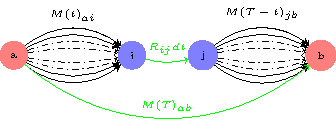
\includegraphics[width=\linewidth]{Fig1.pdf}
     \titlecaption{Phylo-EM Model}
     {Phylo-EM, a special expectation maximization algorithm for maximum likelihood training of substitution rate matrices in sequence alignment. This algorithm can be applied in training hidden substitution models, where the structure of a residue is treated as a hidden variable which evolved during time T \parencite{holmes2002expectation}. $R_{ij}$ is the instantaneous rate of substitution from residue i to j. $M(t)_{ai}$ is the transition matrix from residue a to i, $M(T-t)_{jb}$ is the transition matrix from residue j to b. $M(T)_{ab}$ is the transition matrix from observed residue a to b containing all possible paths.\par}
     \end{minipage}
\end{figure}

\subsection{Maximum Likelihood Estimators}
If there is sequence I, J and alignment A, then their joint probability can be represented as: 
\begin{equation*} 
 P(I,J,A;\theta)  = \prod_{i}\prod_{j} P_{i,j} \pi_{i} = \prod_{i}\prod_{j} e^{R_{i,j}} \pi_{i} 
\end{equation*}

\noindent Where $\pi_i$ are the codon frequencies. $P_{i,j}$ is the substitution rate from i to j ($1 <= i <= 61$, $1 <= j <= 61$), which is denoted as the exponential of the rate matrix $R_{ij}$. If the true alignment of sequences I and J is known, this algorithm offers a solution to the maximum likelihood formula: 
\begin{gather*}
\hat{\theta} = \underset{\theta}{argmax}L(I,J,A|\theta)
\end{gather*}
where $\theta$ represents our parameter set $\{\sigma s, \omega\}$. $\sigma$s include six nucleotide exchangeabilities from the GTR model, $\omega$ measures the selective pressure on non-synonymous substitutions from the MG94 model. A represents the alignment between homologous sequences I and J. Branch length $\tau$ can be derived from the six $\sigma$s and base frequencies. The maximum likelihood estimate of  $\{\sigma s, \omega\}$ from Phylo-EM are: 
\begin{gather*}
\scalebox{.9}{$C_{ij} = \frac{1}{M(T)}\left (\int_{0}^{T} M(t)(R_{ij}dt)M(T-t)\right )$}\\
\scalebox{.9}{$W_{ij} = \frac{1}{M(T)}\left (\int_{0}^{T} M(t)(dt)M(T-t)\right)$} \\
\scalebox{.9}{$\omega: A_w=\sum_{i}\sum_{j,nsyn}C_{ij}, B_w=\sum_{i}\sum_{j,nsyn}W_{i}R_{i,i}$}\\
\scalebox{.9}{$\sigma: A_\sigma=\sum_{i}\sum_{j,\sigma}C_{ij}, B_\sigma=\sum_{i}\sum_{j,\sigma}W_{i}R_{i,i}$}\\
\hat{\omega} = A_w/B_w \\
\hat{\sigma} = A_\sigma/B_\sigma
\end{gather*}
where $C_{ij}$ represents the expected number of times the transition $i \rightarrow j$, $W_{i}$ is the expected amount of time that the system spent in state i. They are expectations taken over the posterior distribution of Markov trajectories conditional on D. $A_w$, $B_w$, $A_\sigma$, $B_\sigma$ are calculated within the E-step: where $A_w$ is the expectation of the total number of non-synonymous substitution events, and $B_w$ is the expected amount of time spent on the non-synonymous substitution events. $A_\sigma$ is the expectation of the total number of events related to six nucleotide exchange events, and $B_\sigma$ is the expected amount of time spent on the corresponding nucleotide exchange events respectively. The estimates of omega and six $\sigma$s are calculated by setting the derivatives of the log likelihood function to zero in the M-step. 

\subsection{Expectation Maximization}
EM algorithm is an iterative method of finding local maximum likelihood estimates of parameters in statistical models, where the model depends on unobserved latent variables. The update of parameters is processed through a two-step optimization: 1) E-step generates a log likelihood function of, $Q(\theta|\theta_{t})$, where 
\begin{gather*}
           Q(\theta|\theta_{t}) = \sum_{i}\sum_{j,i\neq j}C_{ij}(\theta_t,D)log R_{ij}(\theta) + \sum_{i}W_{i}(\theta_t,D)R_{i,i}(\theta)
\end{gather*}
and takes the expectations ($C_{ij}, W_{ij}$) over the posterior distribution of Markov chain trajectories conditional on observed data D. The E-step computation takes a space complexity O ($61^6$) (61 sense codons) and time complexity O ($61^4$). 2) M-step computes parameters maximizing the expected log-likelihood found on the E step, and updates the next estimates of current parameters by taking the first derivative of the log likelihood function. 
\begin{gather*}
              \theta_{t+1} = \underset{\theta}{argmax}Q(\theta |\theta_{t})
\end{gather*}
The EM process will not stop until the criterion is satisfied, which is that the root mean square error (RMSE) of parameters are less than a default threshold ($10^{-4}$) in this research. 

\subsection{Parameter Space}
The weight space of model parameters $\{\pi, \omega, \sigma \}$ must be determined beforehand. The idea weight range is wide and biologically reliable. For example, (i) the frequency of nucleotide A ($\pi_A$) is uniformly sampled between 0 and 0.5, and the rest three nucleotides can be obtained via the Chargaff’s rule ($\pi_A=\pi_T$; $\pi_C=\pi_G$). (ii) $\omega$, as a measure of the selective strength bearing on non-synonymous substitutions, is uniformly sampled within the range of (0,0.5] \parencite{zou2021nonsynonymous}. (iii) The six nucleotide exchangeabilities ($\sigma$) follow a gamma distribution with a shape parameter $\alpha$ and a scale parameter $\beta$, where $\alpha$ is the reverse of square of coefficient of variation (CV), and $\beta$ is the mean substitution rate divided by $\alpha$. In order to obtain a relatively wide distribution of $\sigma$ with a lower mean of $\tau$, I choose the mean substitution rate of 0.4 and the CV of 1. Since a lower $\tau$ approximates to the estimates across real species data, and a higher CV tends to reduce the bias from random simulations. All 100 true parameter values are shown in the supplementary table \ref{tab:true_par}.  

\subsection{Initial Parameter Estimate}
Decent initial parameters is the key to reducing the running time of EM convergence. (i) Because of the missing stop codons in the dataset, our initial values of $\pi$ are estimated via an EM method on a multinomial distribution of codon frequencies. The E-step calculates a likelihood function of 61 sense codons, and the M-step updates the nucleotide frequencies by including the expected frequencies of stop codons. (ii) $\sigma$s are estimated through a distance method applied on the GTR model \parencite{felsenstein2004inferring}. Constrained from the neutral assumption of the method, I only seek for the third positional change of each 4-fold degenerate site of each codon. (iii) $\omega$ is approximated by the ratio of observed non-synonymous substitutions to the expected non-synonymous substitutions. The observed substitutions are extracted directly from the sequence pairs. The expected substitutions are calculated by multiplying the number of codons by the expected substitution rates, which can be obtained by setting up the value of $\omega$ equals to 1 in the MG94 model. This removes the purifying selection constraints against the non-synonymous codons.  

\subsection{Simulations}
I conduct 100 simulations for training the GTR+MG94 model within the Phylo-EM method. Each simulation utilizes a random parameter set to generate pseudo sequence pairs, run the EM algorithm, and measure the accuracy of the estimates. Besides, three gradients of codon length \{$10^5$, $10^6$, $10^7$\} are selected for each hundred simulations, due to their similar range compared with the 90 species data from the paper. 

\subsection{Nelder-Mead Algorithm For Derivative-free Optimization}
I compare the Phylo-EM to a numerically optimizing algorithm called Nelder-Mead algorithm, which is a direct search method without necessarily knowing the derivatives with respect to parameters. I find this method in a R package (dfoptim) and conduct 100 identical simulations. 
Notably, I modify the convergence criterion of this package so it stays consistent with the Phylo-EM method, which should be the RMSE of parameters instead of log likelihood between iterations. 


%%%%%%%%%%%%%%%%%%%%%%%%%%%%
\section{Results}
\subsection{Validation}

\pagebreak
\begin{figure}[H]
     \begin{minipage}[t]{1\textwidth}
     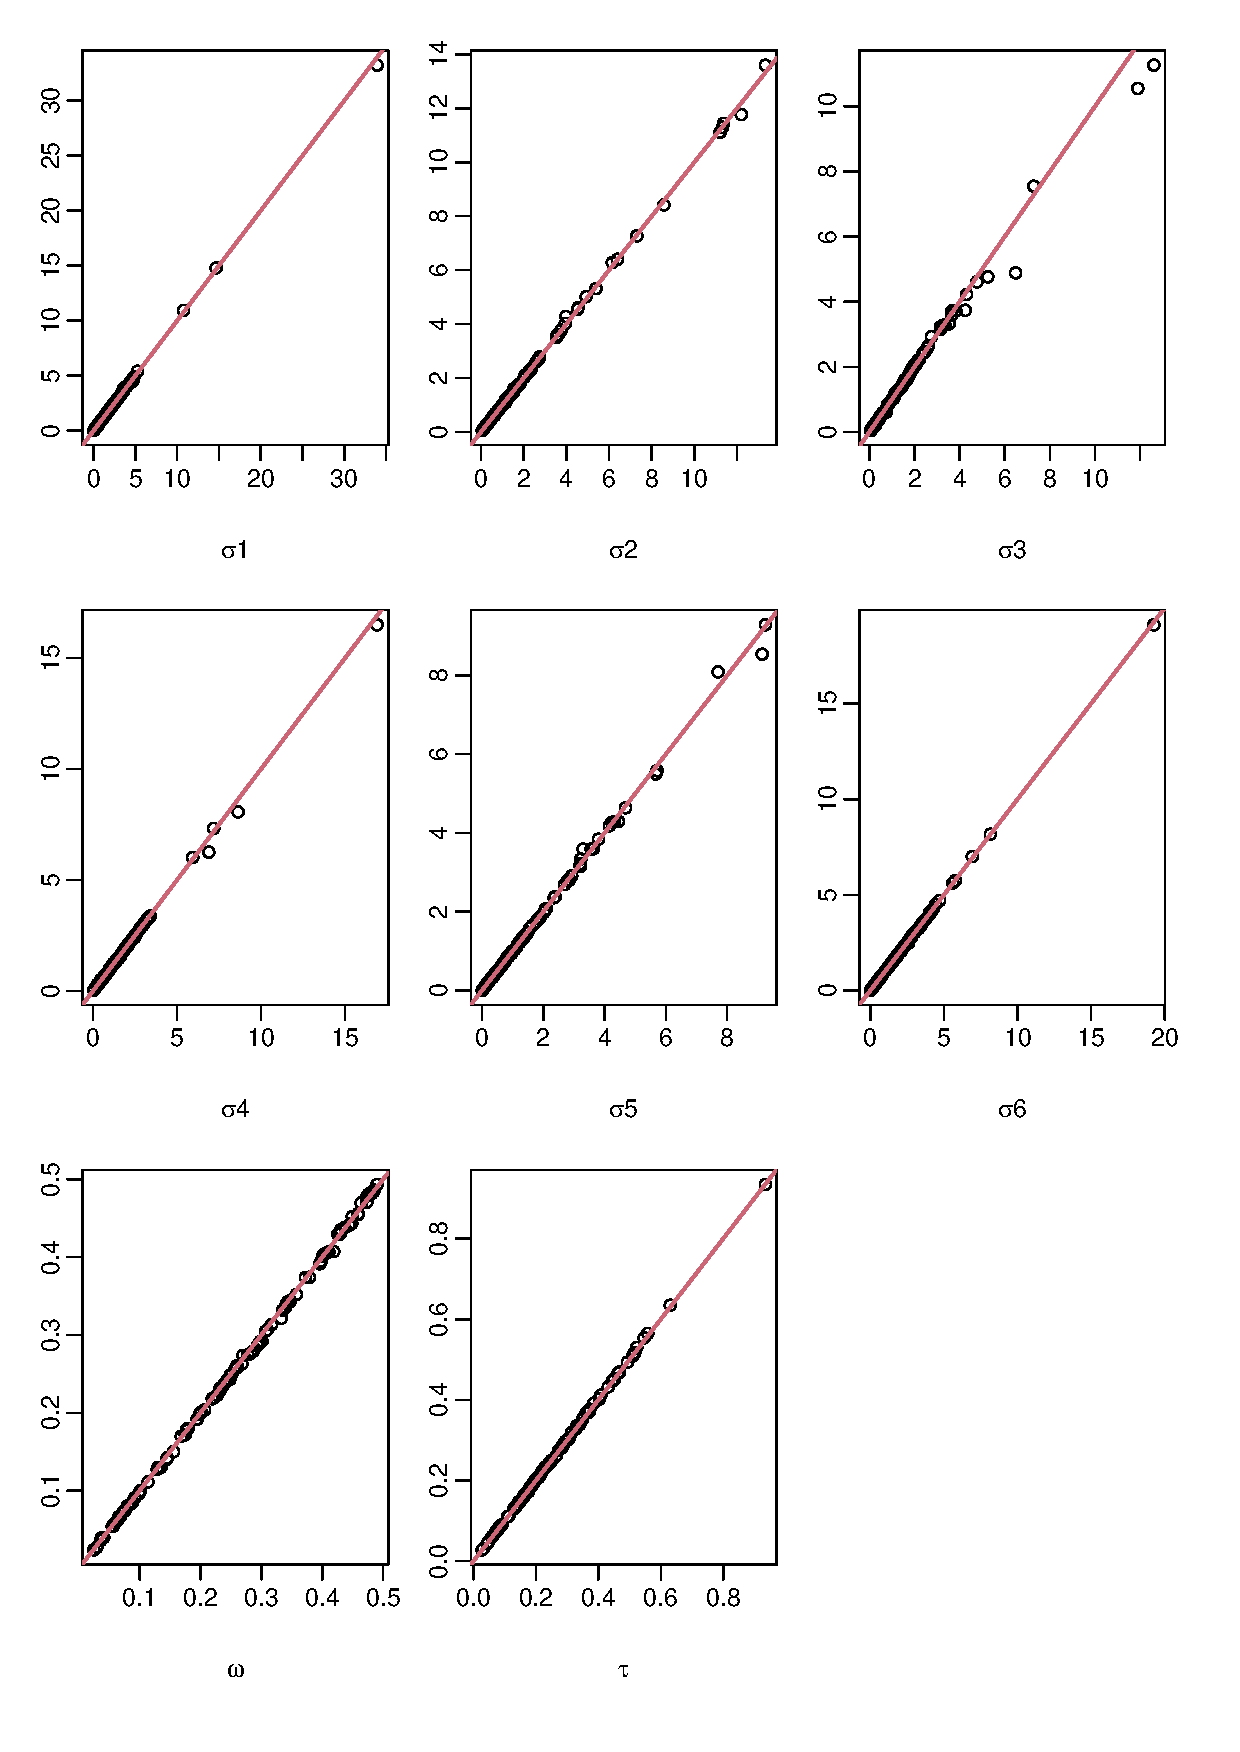
\includegraphics[width=1\linewidth,height=1.2\linewidth]{Fig2.pdf}
     \titlecaption{QQplot of Parameter Estimates in the Codon Length of $10^{5}$ of 100 Simulations}
     { Estimated parameters include six $\sigma$s, $\omega$, and $\tau$. $\{\sigma1$,$\sigma2$,$\sigma3$,$\sigma4$,$\sigma5$,$\sigma6$\} corresponds to the \{$\sigma_{AC}$,$\sigma_{AG}$,$\sigma_{AT}$,$\sigma_{CG}$,$\sigma_{CT}$,$\sigma_{GT}$\}. 
      \par}
     \end{minipage}
\end{figure}

To examine the power of the Phylo-EM algorithm for estimating the parameters extracted from the GTR + MG94 substitution models, we generate a qqplot reflecting the correlation between the true and estimated parameters, including six $\sigma$s, $\omega$, and $\tau$. The diagonal line of Figure 2.2 measures the accuracy between the true and estimated parameters in the codon length of $10^5$. All eight parameter estimates across 100 simulations approximate the true value, except for a few simulated runs. The 100 parameter estimates table is in the APPENDIX \ref{tab:em_par}. \\  
\indent Figure 2.3 displays the root mean squared errors (RMSE) between the true and estimated parameters across 100 simulations in the codon length of \{$10^{5}, 10^{6}, 10^{7}$\}. All three sample sizes are capable of generating accurate parameter estimates with an extremely low RMSE. The mean RMSE values for three sample sizes are 0.061, 0.0168, and 0.007 respectively. And the $95\%$ confidence interval for three sample sizes are [0.042,0.080], [0.011,0.022], and [0.005,0.010]. Clearly, our RMSE value decreases with the increase of sample size across 100 simulations. 
\begin{figure}[H]
     \begin{minipage}[t]{1\textwidth }
     \centering
     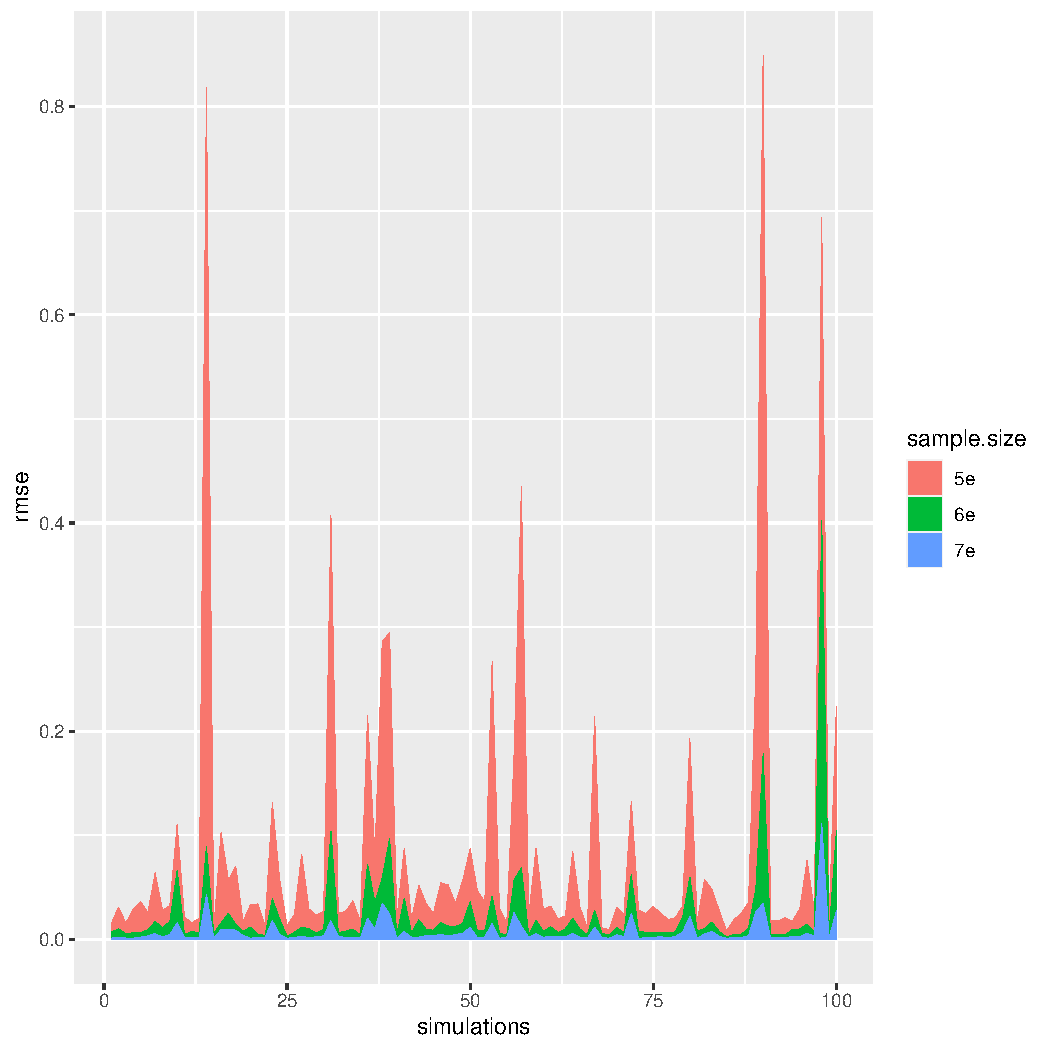
\includegraphics[width=\linewidth]{Fig3.pdf}
     \titlecaption{Root Mean Squared Errors of Parameter Estimates across 100 Simulations in Three Gradient of Sample Size.} {The label of {\{5e,6e,7e\} means the codon length of \{$10^{5}, 10^{6}, 10^{7}$\}respectively}.
      \par}
     \end{minipage}
\end{figure}


\subsection{Data Analysis of 90 Species}
After validating the accuracy of the Phylo-EM, I apply it on a published dataset -- a series of concatenated homologous protein coding sequences from 90 species pairs, including 15 eukaryotic, 6 archaeal, and 69 bacterial clades \parencite{zou2021nonsynonymous}. I generate a data distribution plot of eight parameters from 90 species (Fig 2.4). The mean value of $\sigma_{AC}$, $\sigma_{AG}$, $\sigma_{AT}$,  $\sigma_{CG}$, $\sigma_{CT}$, $\sigma_{GT}$ are 1.23, 2.22, 0.84, 1.16, 2.12, and 0.80 respectively. And the transition rates of nucleotides $\sigma_{AG}$, $\sigma_{CT}$ are higher than the four transversion rates $\sigma_{AC}$, $\sigma_{AT}$,  $\sigma_{CG}$, $\sigma_{GT}$. The mean value of $\omega$, $\tau$ are 0.12 and 0.82. The parameter estimates of 90 species pairs table is in the APPENDIX \ref{tab:90_par}. 
\begin{figure}[H]
     \begin{minipage}[t]{1\textwidth }
     \centering
     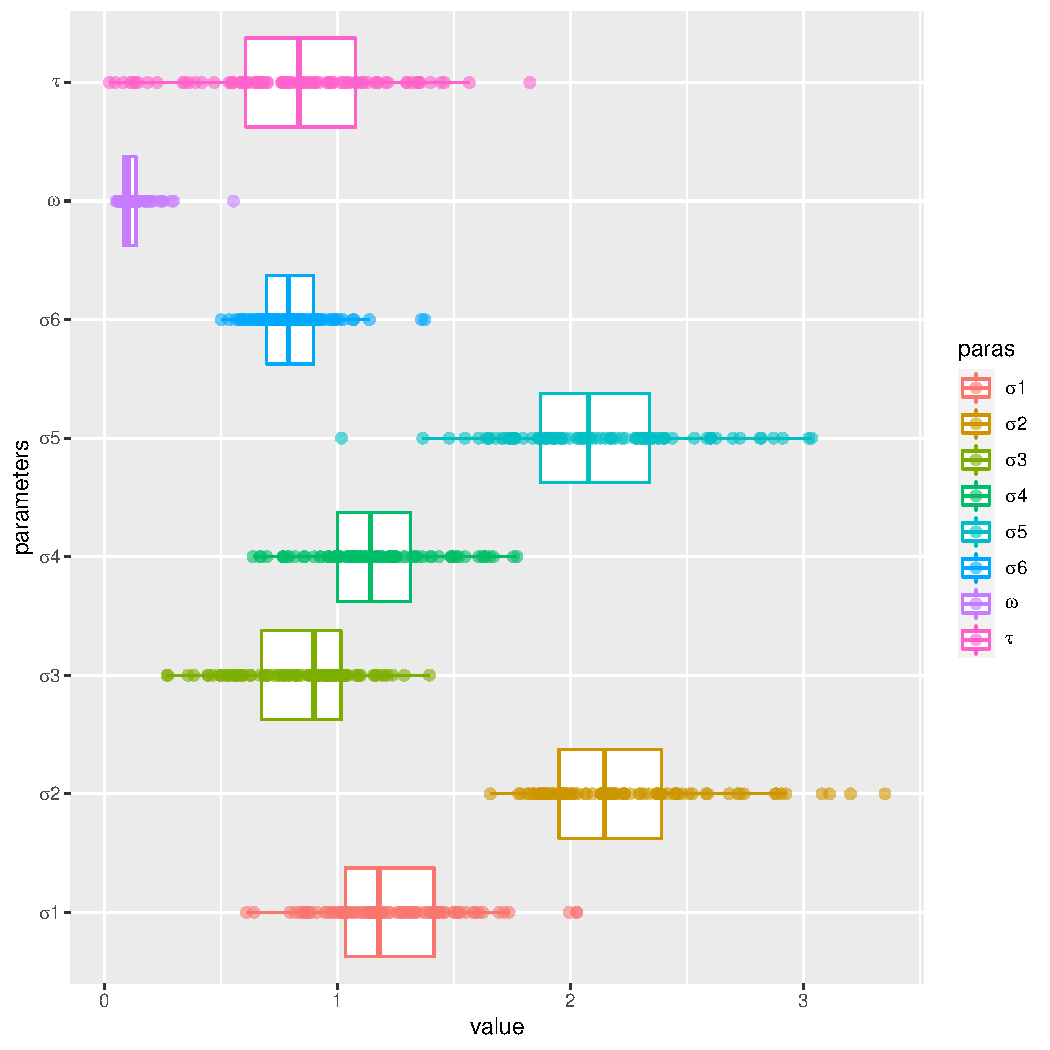
\includegraphics[width=\linewidth]{Fig4.pdf}
     \titlecaption{Distribution of 8 Parameter Estimates from 90 Species Pairs.}
     {{The box boundaries are the 25$\%$ and 75$\%$ quartile. The middle line marks the mean value.}
       \par}
     \end{minipage}
\end{figure}

\indent To further investigate the relationship between $\omega$ and $\tau$, I bootstrap 10 replications in each species with the same sample size. The mean of the standard error of the $\omega$
and $\tau$ of 90 species is 0.0002 and 0.0011, which are extremely small. Figure 2.5 displays a negative correlation between the parameter estimates of $\omega$ and $\tau$ across 90 species. Interestingly, eukaryotic branches (number 1 to 15) have an overall larger $\omega$ and smaller $\tau$, while most prokaryotic branches (number 21 to 90) display the opposite trend. 

\begin{figure}[H]
     \begin{minipage}[t]{1\textwidth }
     \centering
     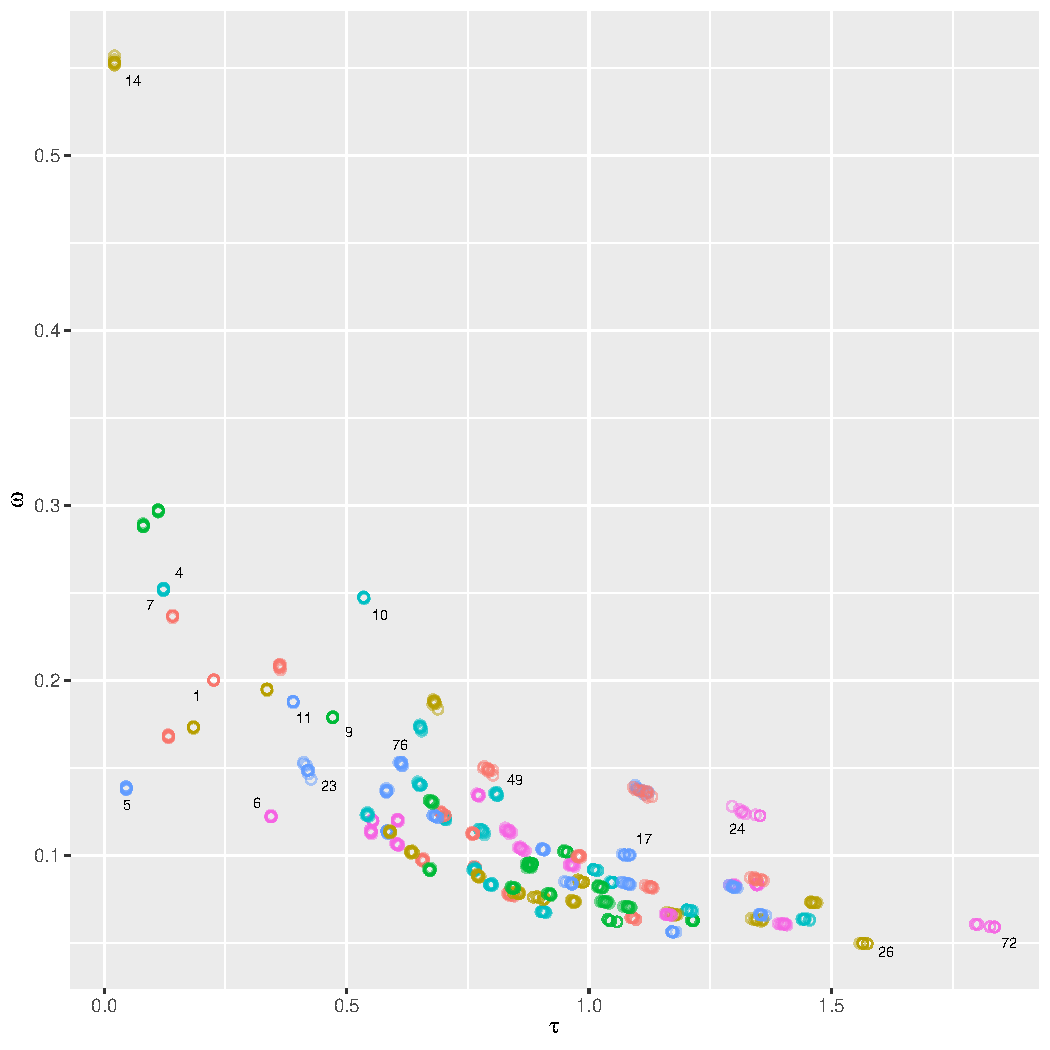
\includegraphics[width=\linewidth]{Fig5.pdf}
     \titlecaption{The Correlation Plot between $\omega$ and $\tau$.}
     {{All species names are represented from number 1 to 90, with 10 bootstrapping replicates in every species. Eukaryotic species taxon names can be found in APPENDIX \ref{tab:spec_name}.} 
      \par}
     \end{minipage}
\end{figure}
  
\subsection{Performance}
Figure 2.6 displays the difference of running EM between using the random and estimated values as initial parameters. The average running time with random values is around 15 iterations, which decreases to 11 iterations by using the estimated ones. And the average time spent on 100 simulations is 20$\%$ less. Moreover, I need at least 5 iterations to pass the true log likelihood threshold by using random initial parameters, reducing to 3 iterations via estimates.  

\begin{figure}[H]
     \begin{minipage}[t]{1\textwidth }
     \centering
     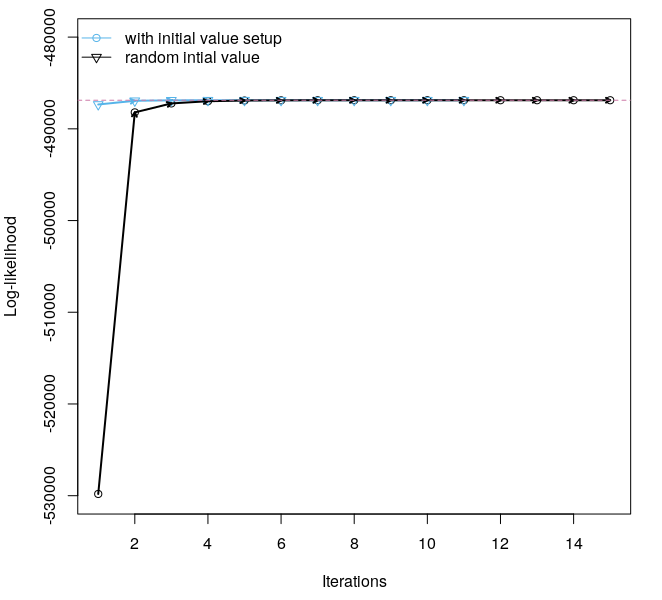
\includegraphics[width=\linewidth]{Fig6.png}
     \titlecaption{Comparison of EM Running Time Difference between Using Random and Estimated Parameters as Initial Values.}
     {{The pink dash line marks the value of the true LL. }
     \par}
     \end{minipage}
\end{figure}

\indent I also assess the performance of the EM and nmkb algorithms for training the MG94 + GTR model. The mean running time of EM for each simulation is around 100 minutes, while the running time of the nmkb derivative-free optimization is about 15 seconds under the same stopping criterion. Figure 2.7 displays a highly overlapped RMSE distribution between the two methods. The mean RMSE value for the EM and nmkb method is 0.061 and 0.062 in the sample size of $10^5$. The parameter estimates from nmkb method can be found in APPENDIX \ref{tab:nmkb_par}. 

\begin{figure}[H]
     \begin{minipage}[t]{1\textwidth }
     \centering
     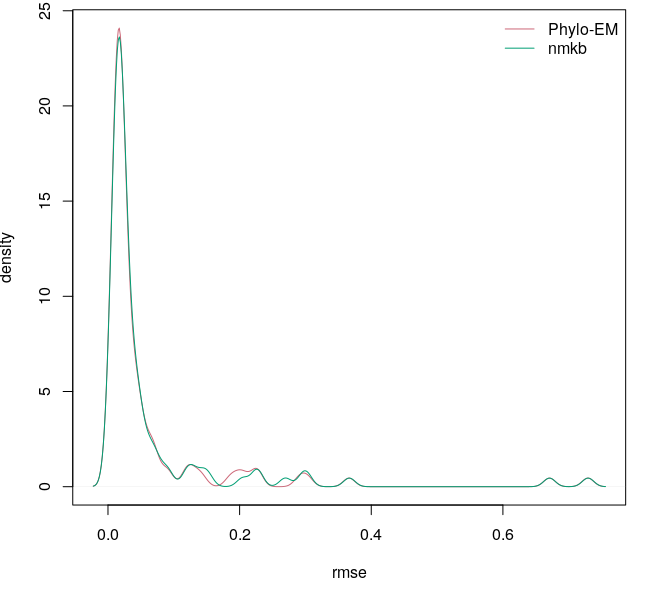
\includegraphics[width=\linewidth]{Fig7.png}
     \titlecaption{The Distribution Plot of RMSE from Phylo-EM and Nmkb Method.}
     {{The green line is nmkb method and the pink line is Phylo-EM method.}
     \par}
     \end{minipage}
\end{figure}

%%%%%%%%%%%%%%%%%%%%%%%%
\section{Discussion}
The EM algorithm proposed by \cite{holmes2002expectation} is an efficient tool of training hidden substitution matrices. I apply this algorithm for simulating the MG94 + GTR models and obtaining the parameter estimates including six nucleotide exchangeabilities $\sigma$, selective pressure on non-synonymous changes $\omega$, and branch length $\tau$. While numerical optimization performs faster than EM for estimating the parameters of the MG94 + GTR model, EM method is still academically useful for its guaranteed increased likelihood, closed form solutions, and compatibility with incomplete datasets \parencite{couvreur1997algorithm}. Especially in the case of complex models (ex. empirical codon model) with a large amount of parameters \parencite{kosiol2007empirical}. \\
\indent Additionally, I apply the Phylo-EM method on 90 species pairs. Figure 2.5 shows that the species carrying a smaller $\omega$ are mostly prokaryotes, where the corresponding branch length $\tau$ are larger. It is still unclear to me that the negative correlation between $\tau$ and $\omega$ is due to biological or technical reasons. Therefore, I propose several explanations here: (i) The effective population size (Ne) of eukaryotes is substantially (by orders of magnitude) smaller than prokaryotes, and consequently, purifying selection is not strong enough to eliminate most of the non-synonymous substitutions compared to the prokaryotes \parencite{sela2016theory}. (ii) Species pairs with a smaller $\tau$ are more likely to be recently diverged, where the existing mutations are still unfixed \parencite{charlesworth2020long}. And those non-synonymous differences lead to an overestimate of $\omega$. (iii) The sequence quality can also be an issue. For instance, The difference of genome sizes across 90 pairwise species tends to cause the discrepancy of the sequence quality. The larger the genome size, the lower the sequence quality normally is \parencite{baker2012novo}. Next, even a list of one-to-one orthologous genes are claimed to be collected for each species, some paralogs are likely to mix into the dataset due to the limitation of the genome annotations and phylogenies \parencite{smith2021new}. Besides, each gene has multiple orthologs that might lead to a different pairwise alignment \parencite{studer2009confident}. \\
\indent In addition to the relationship analysis above, I also found that pairwise species $Thermococcus_{72}$ (ATGC279) and $Lactobacillus_{26}$ (ATGC056) both had a very large $\tau$ (1.8249, 1.5656), while the corresponding value of $\omega$ were close to zero (0.0593, 0.0495). A low $\omega$ suggests that those species are under strong purifying selection but with a high substitution rate in each site, which seems implausible. Since it requires most substitution events are synonymous and the mutational burden falls onto the third position of almost every codon. Therefore, I suspect that the researchers might recover the conserved coding regions from the low-quality sequences, which leads to the over-filtering (artificial selection) of the original dataset, and causes the bias of our parameter estimates. 


\subsection{Limitations}
It is challenging to verify any of the above explanations because: (i) requires us to obtain the effective population size (Ne) of all 90 species pairs. However, the estimation methods of Ne are various and sometimes unreliable \parencite{wang2016prediction}, and most species lack estimated Ne as well. (ii) requires single nucleotide polymorphism (SNPs) data to recognize whether the non-synonymous codon changes are fixed yet \parencite{ochman2003neutral}. Other historical events that can shape the dynamics of substitutions, including Hill-Robertson effect, and background selection are not discussed either \parencite{comeron2008hill}. (iii) demands retrieving the sequencing errors and pulling out the sequencing quality of each alignment. But our 90 pairwise alignments are extracted from various sources, including Ensembl, ATGC, flybase, and OrthoMaM database. Most aligned prokaryotes are extracted from the multiple sequence alignment indirectly, which can also be inaccurate if the phylogenetic trees are misplaced. 

   











%\bibliographystyle{unsrtnat}
%\bibliography{cha1/ref1.bib}
